% Build with XeLaTeX, BibTeX, then XeLaTeX twice.
% Official ICLR 2027 style; measured results remain blank until evaluation.
\documentclass{article}
\usepackage{vendor/iclr2027/iclr2027_conference}
\usepackage{fontspec}
\setmainfont{Times New Roman}
\setsansfont{Times New Roman}
\setmonofont{Times New Roman}
\font\iclrtenhv="Times New Roman/B" at 8pt
\usepackage[protrusion=true,expansion=false]{microtype}
\usepackage{amsmath,amssymb,booktabs,array,graphicx,xcolor,placeins,xurl}
\usepackage[hidelinks]{hyperref}
\urlstyle{same}
\newcommand{\R}{\mathbb{R}}
\newcommand{\E}{\mathbb{E}}
\newcommand{\blank}{\textcolor{gray}{\textemdash}}
\newcommand{\figureblank}[2]{\fbox{\begin{minipage}[c][#1][c]{.94\linewidth}\centering\color{gray}#2\end{minipage}}}
\newcommand{\resultslot}{\par\smallskip{\color{gray}\textit{[Experimental findings.]}}}
\title{SERVE: Semantic Evidence from Return\\Verification for LiDAR Segmentation}
\author{Anonymous authors}
\lhead{Under review as a conference paper at ICLR 2027}
\begin{document}
\maketitle

\begin{abstract}
Semantic segmentation assigns a known class to every LiDAR point, including observations of unfamiliar objects. Detecting these objects requires assessing whether the predicted class is supported by the observation. We introduce Semantic Evidence from Return Verification (SERVE), an end-to-end model that learns this assessment from normal semantic labels and measured ranges. A full-scan encoder represents the observed point, while a separate context encoder predicts a log-range distribution for each known class. The context encoder excludes all returns in the target angular cell, making the measured range a held-out target for prediction. Each class combines appearance support with the likelihood of that measurement. The class with the strongest joint support supplies the semantic label, and its energy supplies the unknown score. Normal labels train both terms through the resulting class probabilities, while a likelihood objective fits the predictive distributions to normal observations. Multiple appearance modes and predictive components accommodate variation within each class. Evaluation on nuScenes and STU examines normal semantic accuracy, real-anomaly detection, high-recall false positives, and inference cost. {\color{gray}\textit{[Experimental findings.]}}
\end{abstract}

\section{Introduction}
\label{sec:intro}
LiDAR semantic segmentation assigns observed points to a fixed set of known classes. An unfamiliar road obstacle must therefore receive one of these labels, even when it differs from every class represented in training. A high class probability expresses a preference among the available labels, leaving open whether the selected class adequately explains the observation. Reliable perception consequently requires both a semantic prediction and an assessment of the evidence supporting it. STU provides a setting for studying this problem through point-level annotations of unexpected objects in real road scenes \citep{stu}.

Normal semantic annotations provide a way to learn this assessment without enumerating future unknown objects. LIDO organizes LiDAR features around semantic prototypes \citep{lido}, PixOOD models multiple normal feature configurations \citep{pixood}, and RbA identifies image regions rejected by known classes \citep{rba}. These methods use learned class support to recognize observations that fall outside the known vocabulary. We investigate an additional source of support: whether a candidate class can predict a physical measurement from the surrounding scene.

The spatial structure of LiDAR observations makes this prediction possible. Neighboring returns constrain how a surface can continue through a local region, and a candidate class further specifies the normal structures expected there. Under a road hypothesis, nearby ground returns constrain the range along a held-out direction. A measurement that departs from that continuation weakens the road hypothesis. A vehicle class can provide an alternative explanation for a normal car at the same location. The relevant decision is therefore whether a single known class supports both the observed point features and the measured range (Figure~\ref{fig:motivation}).

\begin{figure}[t]
\centering
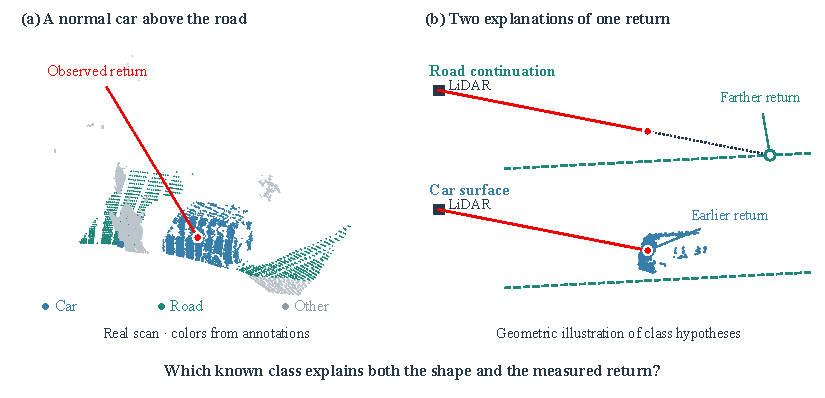
\includegraphics[width=\linewidth]{figures/motivation.pdf}
\caption{A normal explanation requires support for the same class. Both illustrative cases share identical appearance support. When appearance and return evidence favor the same class, its joint support is strong. When they favor different classes, both joint supports are weak and the unknown score rises. Return support is the predictive density at the observed range divided by a common bound $M$. Class probabilities follow by normalizing the joint supports.}
\label{fig:motivation}
\end{figure}

To obtain this measurement evidence, the predictor must infer the target range from surrounding observations. SERVE excludes every return in the target angular cell before combining neighboring measurements. Its full-scan semantic encoder separately preserves the observed geometry and point details. Because normal objects vary in pose, shape, and visibility, the context encoder predicts a distribution of plausible ranges for each class. Evaluating this distribution at the measured range supplies class-specific observation support. A normalized density accounts for both prediction error and predictive spread.

The connection to semantic learning determines how SERVE uses this support. Class-conditioned reconstruction supports open-set recognition and segmentation \citep{c2ae,coreseg}, while semantic representations guide multi-category anomaly reconstruction \citep{sedir}. SERVE places the likelihood of a held-out measurement directly inside the supervised pointwise class decision. Appearance support and measurement support are multiplied within each class, so the selected class must account for both. Normal semantic labels train this joint class competition, and a likelihood objective fits the predicted distributions to measured ranges. The measurement target remains fixed as the semantic representation learns.

SERVE thus learns semantic segmentation and unknown recognition through the same class-support function. Its central mechanism is a class-conditioned prediction of held-out LiDAR range whose likelihood participates in learning the semantic decision. We evaluate whether this coupling preserves normal semantic accuracy while detecting unknown points that an appearance-based classifier confidently assigns to known classes. Measuring these outcomes together with high-recall false positives and full-scan computation connects the proposed mechanism to its practical value for perception.

\section{Related Work}
\label{sec:related}
\paragraph{Unknown recognition within semantic perception.}
Confidence and energy scores assess unknown inputs through a classifier's outputs \citep{msp,energy}. Joint energy models connect classification and generative learning through shared class energies \citep{jem}. Dense open-set methods develop this connection through class rejection, feature distributions, and joint discriminative and generative objectives \citep{rba,pixood,densehybrid}. In LiDAR, LIDO learns compact normal-class features \citep{lido}, and hierarchical Gaussian mixtures model class-conditional feature uncertainty \citep{hgmm}. Generated or auxiliary unknown observations provide another source of supervision, including resized objects, diverse synthetic objects, diffusion-generated examples, and distribution-prior learning \citep{real,lion,doodle,ndp,rel}. SERVE learns appearance and measurement support from normal semantic labels and measured ranges.

\paragraph{Class-conditioned reconstruction and anomaly detection.}
Reconstruction assesses an observation by comparing it with a learned normal representation. Image resynthesis makes this comparison through a generated image conditioned on semantic predictions \citep{resynthesis}. C2AE learns class-conditioned reconstruction for open-set recognition \citep{c2ae}, and CoReSeg uses the smallest class-conditioned reconstruction error to reject unknown pixels in dense labeling \citep{coreseg}. UniAD controls information transfer when reconstructing normal features \citep{uniad}. In 3D, IMRNet detects object anomalies through iterative masked reconstruction \citep{imrnet}, while SeDiR uses object-category semantics and geometric attention to organize multi-category feature reconstruction \citep{sedir}. In SERVE, each class predicts a held-out range distribution, and its likelihood participates in the supervised pointwise class decision.

\paragraph{Context prediction and probabilistic support.}
Excluding the prediction target makes surrounding observations the source of predictive information. Blind-spot denoising uses this principle for self-supervision \citep{noise2self,blindspot,pn2v}, and conditional neural processes predict distributions at query locations from observed context \citep{cnp,anp}. Point-cloud pretraining uses prediction objectives to learn representations \citep{pointmae,ponder,sonata}, while probabilistic LiDAR fields model range distributions for mapping \citep{plink}. A logarithmic scoring rule provides a direct objective for fitting such distributions \citep{proper}. Studies of generative likelihood show that unknown-sample rankings depend on the observation representation and scoring rule \citep{likelihood,perfectdensity}. SERVE uses predictive likelihood as measurement evidence within each semantic class and trains the resulting joint support through normal class supervision.

\section{Semantic Evidence from Return Verification}
\label{sec:method}
\subsection{Semantic Decisions from Joint Class Support}
\label{sec:joint}
SERVE maps a single scan to a semantic label and an unknown score for every return. Let the scan be $X=\{(\mathbf{x}_i,I_i)\}_{i=1}^{N}$, where $\mathbf{x}_i\in\R^3$ is a return in the scan coordinate frame and $I_i$ is its intensity. Define range $r_i=\|\mathbf{x}_i\|_2$, direction $\boldsymbol\omega_i=\mathbf{x}_i/r_i$, and log range $z_i=\log r_i$. The known vocabulary is $\mathcal C=\{1,\ldots,C\}$. Training provides a known class $y_i$, or an allowed set $Y_i\subseteq\mathcal C$ when a source label corresponds to several target classes. The outputs are $\hat y_i\in\mathcal C$ and $u_i\in\R$.

For each candidate class, we compute appearance support $a_{ic}\in(0,1]$ and a conditional density $p_{ic}=p_\theta(z_i\mid C_i,\boldsymbol\omega_i,c)$, where $C_i$ contains surrounding returns and excludes the target angular cell. A common upper bound $M$ on the density defines measurement support $b_{ic}=p_{ic}/M$. The joint support and corresponding energy are
\begin{equation}
 v_{ic}=a_{ic}b_{ic},\qquad
 E_{ic}=-\log v_{ic}=s_{ic}+g_{ic},\qquad
 s_{ic}=-\log a_{ic},\quad g_{ic}=\log M-\log p_{ic}.
 \label{eq:energy}
\end{equation}
Both outputs follow from these class energies:
\begin{equation}
 \hat y_i=\arg\min_{c\in\mathcal C} E_{ic},\qquad
 u_i=\min_{c\in\mathcal C} E_{ic}.
 \label{eq:outputs}
\end{equation}
The label identifies the best-supported class. The unknown score measures the weakness of that class's joint support, even when it wins by a large margin over other classes.

\begin{figure}[htbp]
\centering
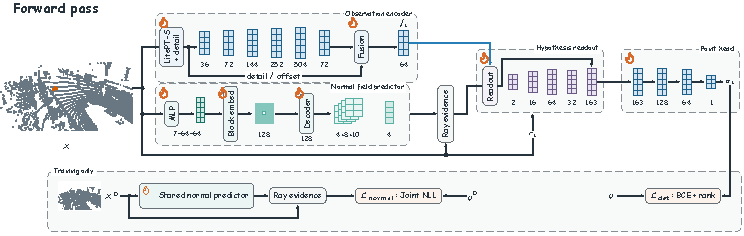
\includegraphics[width=\linewidth]{figures/method.pdf}
\caption{SERVE architecture. The full-scan branch combines voxel features with point details and projects them to a 48-dimensional embedding. Shared class vectors organize appearance centers and query independently encoded surrounding cells. Within the prediction branch, target exclusion precedes cross-cell attention; the actual target range enters only the subsequent density evaluation. Evidence combines within each class before semantic labeling and unknown scoring. Dashed paths show the joint classification and predictive likelihood objectives; auxiliary losses are specified in Equation~\eqref{eq:loss}. The input is a real LiDAR scan, colored by height and cropped to $2.5$--$35$\,m range and $-3$--$8$\,m height. Density curves are schematic.}
\label{fig:method}
\end{figure}

\paragraph{A common class must explain both observations.}
Combining the two supports within each class is essential to the decision rule. Independent maximization could select different classes for appearance and measurement, since
\begin{equation}
 \max_c(a_{ic}b_{ic})\;\leq\;
 (\max_c a_{ic})(\max_c b_{ic}).
 \label{eq:agreement}
\end{equation}
For example, appearance supports $(0.9,0.1)$ and measurement supports $(0.1,0.9)$ give a maximum joint support of $0.09$, whereas independently choosing each maximum gives $0.81$. Equation~\eqref{eq:energy} retains this disagreement: a class receives strong joint support when both its appearance representation and its range prediction support the observation.

\subsection{Multimodal Appearance Support}
\label{sec:appearance}
Appearance support represents the observed geometry across the complete scan. A LitePT-S backbone \citep{litept} encodes this geometry after $5$\,cm voxel aggregation. To preserve differences between returns in the same voxel, a point-level encoder embeds each return's coordinates, intensity, and offset from its voxel center. Concatenating this embedding with the decoded voxel feature produces $\mathbf h_i\in\R^D$, with $D=48$.

Normal objects within a class can have different observed shapes and point densities. We represent this variation with a shared class vector $\mathbf q_c$ and $A=4$ learned offsets $\boldsymbol\delta_{cm}$. The resulting appearance centers and support are
\begin{equation}
 \mathbf t_{cm}=\sqrt D\,\frac{\mathbf q_c+\boldsymbol\delta_{cm}}
 {\|\mathbf q_c+\boldsymbol\delta_{cm}\|_2},\qquad
 a_{ic}=\frac{1}{A}\sum_{m=1}^{A}
 \exp\!\left(-\frac{\|\mathbf h_i-\mathbf t_{cm}\|_2^2}{D\tau}\right),
 \label{eq:appearance}
\end{equation}
where $\tau=0.2$. Equal center norms, temperature, and mode counts provide a common scale across classes. The same $\mathbf q_c$ conditions the range predictor, connecting each class's appearance representation to the measurements it predicts.

\subsection{Predicting Returns from Target-Excluded Context}
\label{sec:prediction}
\paragraph{Information available to the predictor.}
Measurement support evaluates a prediction formed from neighboring returns. We partition azimuth and elevation into nonoverlapping $0.5^\circ$ cells and encode each cell independently. A pointwise encoder maps coordinates, intensity, and direction to features, which are aggregated by mean and maximum pooling within the cell. For each target cell, class queries attend to eight neighboring offsets at each of two radii, one and three cells. Excluding the target cell's token makes these neighbors the sole source of observed context. Two shared attention layers of width $48$ process the class queries.

Independent cell encoding places the exclusion before any cross-cell interaction. The query supplies the target cell's angular position and the candidate class, while the context supplies the neighboring measurements. The target range is reserved for evaluating the predictive density. The appearance path separately processes the complete scan, as shown in Figure~\ref{fig:method}. Applying the same construction to every cell allows all predictions to share the point encoder and context projections.

\paragraph{A distribution of plausible normal returns.}
For each target cell $j$ and class $c$, the predictor outputs $K=3$ mixture weights $w_{jck}$, mean parameters, and scales $\sigma_{jck}$. Let $(d_a,d_e)$ be a ray's azimuth and elevation offsets from the cell center, normalized by the half-cell width, and define
\begin{equation}
 \boldsymbol\phi_i=(d_a,d_e,d_a^2,d_ad_e,d_e^2),\qquad
 \mu_{ick}=\bar z_{C_j}+\alpha_{jck}
                  +\boldsymbol\beta_{jck}^{\mathsf T}\boldsymbol\phi_i.
 \label{eq:surface}
\end{equation}
Here $\bar z_{C_j}$ averages the mean log ranges of available neighboring cells. Learned quadratic coefficients express local range variation across rays. The scale is $\sigma_{jck}=\sigma_{\min}+\operatorname{softplus}(\rho_{jck})$, with $\sigma_{\min}=10^{-3}$, and mixture weights sum to one within each class.

The conditional density is a Student-$t$ mixture with three degrees of freedom:
\begin{equation}
 p_{ic}=\sum_{k=1}^{K}w_{jck}\,
 \frac{2}{\pi\sqrt3\,\sigma_{jck}}
 \left(1+\frac{(z_i-\mu_{ick})^2}{3\sigma_{jck}^2}\right)^{-2}.
 \label{eq:density}
\end{equation}
The mixture components represent alternative local range patterns, and their learned scales describe the spread of plausible observations. Context determines these parameters before Equation~\eqref{eq:density} is evaluated at the held-out measurement. The appearance centers and predictive components therefore represent complementary aspects of normal variation.

\paragraph{Measurement support includes predictive concentration.}
Each component is bounded above by $M=2/(\pi\sqrt3\,\sigma_{\min})$, so the mixture yields $0<b_{ic}\leq1$. Equation~\eqref{eq:energy} retains the scale normalization of the density. At a component mean, increasing its scale by a factor of ten raises its negative log density by $\log 10$. A broad prediction therefore carries a cost as well as accommodating a wider range of returns. For a completely isolated target cell, we set $b_{ic}=1$ for all classes, giving the appearance-based decision. The predicted variable is the log range of an existing return, with density defined relative to $d(\log r)$.

\subsection{Learning Verification through Normal Class Competition}
\label{sec:learning}
The class distribution used for semantic learning is
\begin{equation}
 P_\theta(c\mid X,i)=\frac{\exp(-E_{ic})}{\sum_{d\in\mathcal C}\exp(-E_{id})},\qquad
 \ell_{\mathrm{joint},i}=-\log\sum_{c\in Y_i}P_\theta(c\mid X,i).
 \label{eq:jointloss}
\end{equation}
For a fine label $Y_i=\{y_i\}$ with available neighboring cells, normal semantic supervision trains the observed appearance and the measurement prediction to favor the same class. In particular,
\begin{equation}
 \frac{\partial\ell_{\mathrm{joint},i}}{\partial\log p_{ic}}
 =P_\theta(c\mid X,i)-\mathbf1[c=y_i].
 \label{eq:gradient}
\end{equation}
Increasing the true class's measurement likelihood reduces the classification loss, while increasing a competing class's likelihood raises it. The predictive branch therefore receives semantic supervision through the same class decision as the appearance branch.

Class competition compares candidate explanations, and a predictive likelihood objective fits each class's distribution to its normal measurements. The context states produce class logits $\eta_{ic}$, which define a mixture restricted to the allowed label set,
\begin{equation}
 \pi_{ic}^{Y}=\frac{\exp\eta_{ic}}{\sum_{d\in Y_i}\exp\eta_{id}}\quad(c\in Y_i),\qquad
 \ell_{\mathrm{pred},i}=-\log\sum_{c\in Y_i}\pi_{ic}^{Y}p_{ic}.
 \label{eq:predloss}
\end{equation}
For a fine label, this objective is the negative log likelihood (NLL) under the true class. For a coarse label, it fits the allowed-class mixture to the measured range. The logarithmic score rewards predictive distributions that fit the normal observations \citep{proper}, while a context-class loss supervises the total probability assigned to $Y_i$.

The appearance representation also receives direct semantic supervision. Replacing $E$ with $s$ in Equation~\eqref{eq:jointloss} gives an appearance classification loss on every reliably labeled point. A compactness loss additionally increases absolute appearance support for the allowed classes,
\begin{equation}
 \ell_{\mathrm{compact},i}=-\log\left(\frac{1}{|Y_i|}\sum_{c\in Y_i}a_{ic}\right).
 \label{eq:compact}
\end{equation}
The training objective is
\begin{equation}
 \mathcal L=\mathcal L_{\mathrm{joint}}
 +0.5\mathcal L_{\mathrm{appearance}}
 +0.05\mathcal L_{\mathrm{compact}}
 +0.2\mathcal L_{\mathrm{pred}}
 +0.2\mathcal L_{\mathrm{context}}.
 \label{eq:loss}
\end{equation}
We balance classification losses over the distinct allowed label sets present in a frame. Predictive likelihood and compactness are point averages. Up to $4{,}096$ normally labeled points per frame supervise joint verification, while the appearance loss covers all reliable normal labels. The complete scan supplies the input. Appendix~\ref{app:training} specifies these reductions and the source-to-target schedule.

\paragraph{Inference and a normal reference scale.}
A single scan supplies the appearance features and context predictions. Neighboring tokens are encoded once, and class parameters are shared across angular cells. Evaluating each class density at the original point's range yields the label and raw unknown score in Equation~\eqref{eq:outputs}. A strictly increasing transform fitted to normal development scores then expresses $u_i$ on a common normal-reference scale. Because the transform is shared across classes and preserves score order, it retains the ranking defined by joint class support.

\section{Experiments}
\label{sec:experiments}
The evaluation follows the role of measurement evidence in SERVE. Normal semantic accuracy measures its effect on known-class decisions. Real-anomaly detection tests whether it identifies unknown points that an appearance-based classifier assigns to known classes. High-recall false positives and inference cost then characterize the operating conditions under which this additional evidence is useful.

\subsection{Data, Training, and Evaluation}
\paragraph{Normal supervision.}
Training combines broad normal observations from nuScenes with target-sensor observations from STU. nuScenes \citep{nuscenes} supplies $28{,}130$ training scans from $700$ scenes and a scene-disjoint development set of $6{,}019$ scans from $150$ scenes. STU sequence 206 supplies $449$ normal training scans, and sequence 201 supplies $682$ normal development scans. The output vocabulary contains the $19$ STU normal classes. Coarse nuScenes labels specify sets of compatible target classes, and additional source annotations refine selected bicycle, parking, and building points. Semantic supervision uses reliable normal labels within $2.5$--$50$\,m. All recorded returns remain available as input, including points with ambiguous labels.

\paragraph{Optimization.}
The backbone starts from official nuScenes-pretrained LitePT-S weights. All other parameters are initialized randomly. Source training comprises two passes over nuScenes, followed by eight passes over sequence 206 with one source replay scan per four target scans. AdamW uses an effective batch size of two, weight decay $0.005$, $3\%$ linear warmup, and cosine decay to $5\%$ of the peak rate. The source peak rates are $10^{-4}$ for the backbone and $8\times10^{-4}$ for new parameters; target rates are $3\times10^{-5}$ and $2\times10^{-4}$. Selection uses normal-development mean intersection-over-union (mIoU), with the normal objective breaking ties. The independent controls use the same initial weights, data order, augmentations, and update budget.

\paragraph{Evaluation.}
Normal perception is evaluated by per-class IoU and mIoU on sequence 201, using the classes represented in its ground truth. STU's real-anomaly validation and hidden test sets supply average precision (AP), area under the receiver operating characteristic curve (AUROC), and the normal false-positive rate at $95\%$ anomaly recall (FPR95). These metrics use the official distance, label, and anomaly-instance rules \citep{stu}, including the official set of normal points in the false-positive denominator. Recall at matched normal false-positive rates of $1\%$ and $5\%$ further compares unknown detection under equal false-alarm budgets. Full-scan latency and peak memory quantify the associated computation on a common device.

\subsection{Normal Perception and Real-Anomaly Segmentation}
\label{sec:benchmark}
Table~\ref{tab:main} evaluates semantic accuracy and unknown detection together because measurement evidence influences both outputs. SERVE and an independently trained appearance model use the same backbone, normal data, and training budget. Their comparison measures the change in perception obtained by introducing class-conditioned return verification.

Published STU results provide an external performance reference. LIDO uses MinkowskiNet trained on SemanticKITTI \citep{lido}. The STU implementations of MC dropout, RbA, MaxLogit, and deep ensembles use Mask4Former-3D trained on SemanticKITTI, Panoptic-CUDAL, and the STU normal training split \citep{stu}. Table~\ref{tab:main} reports these methods' original results alongside the comparison using matched nuScenes and STU normal data.

\begin{table}[htbp]
\caption{Normal perception and real-anomaly segmentation. All metrics are percentages. The first group uses matched normal data and training budgets; dashes reserve pending results. Published results in the second group retain their original training resources; n/r denotes an unreported normal-semantic result.}
\label{tab:main}
\centering\small\setlength{\tabcolsep}{3.5pt}
\begin{tabular}{lrrrrrrr}
\toprule
 & 201 & \multicolumn{3}{c}{STU validation} & \multicolumn{3}{c}{STU test}\\
\cmidrule(lr){3-5}\cmidrule(lr){6-8}
Model & mIoU$\uparrow$ & AP$\uparrow$ & AUROC$\uparrow$ & FPR95$\downarrow$ & AP$\uparrow$ & AUROC$\uparrow$ & FPR95$\downarrow$\\
\midrule
Appearance only & \blank & \blank & \blank & \blank & \blank & \blank & \blank\\
Separate objectives & \blank & \blank & \blank & \blank & \blank & \blank & \blank\\
SERVE & \blank & \blank & \blank & \blank & \blank & \blank & \blank\\
\midrule
MC dropout \citep{stu} & n/r & 0.17 & 65.76 & 79.82 & 0.11 & 61.51 & 82.37\\
RbA \citep{stu} & n/r & 1.64 & 73.00 & 100.00 & 0.81 & 66.38 & 100.00\\
MaxLogit \citep{stu} & n/r & 2.02 & 87.27 & 68.76 & 0.95 & 84.53 & 81.49\\
Deep ensemble \citep{stu} & n/r & 6.94 & 90.93 & 37.34 & 5.17 & 86.74 & 58.05\\
LIDO \citep{lido} & n/r & 27.53 & 95.05 & 34.86 & 14.99 & 93.67 & 34.29\\
\bottomrule
\end{tabular}
\end{table}

\subsection{Effect of Observation Evidence on Semantic Decisions}
\label{sec:mechanism}
To isolate the role of measurement evidence in semantic learning, the separate-objectives control trains classification using appearance support while retaining the predictive objective, shared class parameters, and joint inference score. Its comparison with SERVE tests the effect of using measurement support during class competition. The independently trained appearance model provides a common reference for examining which pointwise decisions change.

For unknown points, the reference classifier defines a fixed subset whose maximum class probability is at least $0.9$. Recall on this subset measures recovery of confident semantic misrecognitions. At each false-positive rate, we match point identities across models and count recovered and lost unknown points. On normal points, the same analysis counts corrected and newly introduced semantic errors, with per-class IoU exposing the distribution of these changes. Table~\ref{tab:coupling} and Figure~\ref{fig:decisions} join these two views of observation verification.

\begin{figure}[htbp]
\centering
\figureblank{1.12in}{Normal-class IoU changes and unknown recall at matched false-positive rates}
\caption{Effect of verification on semantic decisions and unknown recognition. Left: per-class IoU relative to the independently trained appearance model. Right: recall of confidently misrecognized unknown points at matched normal false-positive rates. The same reference model defines the subset for every method.}
\label{fig:decisions}
\end{figure}

\begin{table}[htbp]
\caption{Changes in pointwise decisions relative to the appearance model. Corrected and introduced normal errors are percentages of all evaluated normal semantic points. Unknown recall is measured on the fixed subset confidently assigned a normal class by the reference model, at matched normal false-positive rates.}
\label{tab:coupling}
\centering\small
\begin{tabular}{lrrrr}
\toprule
 & \multicolumn{2}{c}{Normal semantic errors} & \multicolumn{2}{c}{Unknown recall$\uparrow$}\\
Model & Corrected$\uparrow$ & Introduced$\downarrow$ & at $1\%$ FPR & at $5\%$ FPR\\
\midrule
Appearance only & & & \blank & \blank\\
Separate objectives & \blank & \blank & \blank & \blank\\
SERVE & \blank & \blank & \blank & \blank\\
\bottomrule
\end{tabular}
\end{table}

\subsection{Predictive Quality, Sparse Returns, and Computation}
\label{sec:quality}
Measurement support depends on how well the predicted distributions describe normal returns. We examine held-out log likelihood, the coverage and width of $90\%$ predictive intervals, and mixture-component use. Coverage measures how often a normal return falls within the predicted interval, while width measures how concentrated that prediction is \citep{proper}. Stratifying these quantities by range and angular-cell return count reveals how predictive quality varies with observation sparsity. Applying the same strata to anomaly recall and normal false positives relates prediction quality to detection behavior.

Figure~\ref{fig:qualitative} examines this relationship at individual returns. Normal and unfamiliar objects with similar appearance-based class confidence are shown alongside their class-conditioned range distributions. The measured range then identifies which candidate predictions support the observation. Computational measurements cover scan preparation, semantic encoding, context prediction, and pointwise scoring, with peak memory measured under the same execution conditions for each model.

\begin{figure}[htbp]
\centering
\figureblank{1.12in}{Observed scans, class predictions, unknown scores, and held-out range distributions}
\caption{Class explanations at observed returns. Each selected point is accompanied by the predicted range distributions for the most relevant known classes and its measured range. Normal sparse objects and confidently misrecognized unknown objects are presented with the same visualization scale.}
\label{fig:qualitative}
\end{figure}

\section{Conclusion}
SERVE connects LiDAR semantic decisions to predictions of measured range. Each known class receives appearance support from the full scan and measurement support from a context-conditioned distribution over a held-out return. Normal semantic labels train their joint support through class competition, while a likelihood objective fits the predictive distributions to normal measurements. The resulting class energy supplies both semantic labels and unknown scores, linking the recognition of known objects to the evidence supporting their classification.
\resultslot

\FloatBarrier
\section*{AI Use Statement}
We used OpenAI Codex for literature retrieval and synthesis, research-question refinement, model formulation, mathematical derivations, experiment design, data processing and annotation review, implementation, debugging, and analysis of development results. Manuscript assistance included drafting, editing, reference verification, method naming, diagrams, and typesetting. Verification used source texts for method comparisons, implementation checks for the formulation, and numerical and real-scan tests for the computations. The authors are responsible for the submitted text, claims, code, and data artifacts.

\section*{Reproducibility Statement}
Section~\ref{sec:method} defines the class energies and training objectives. Appendix~\ref{app:architecture} specifies the context construction and predictive distribution, Appendix~\ref{app:training} gives supervision and optimization details, and Appendix~\ref{app:evaluation} defines the evaluation reductions. The experiments use nuScenes and STU with the stated scene and sequence assignments.

\bibliography{paper}
\bibliographystyle{vendor/iclr2027/iclr2027_conference}

\clearpage
\appendix
\section{Predictive Architecture and Decision Function}
\label{app:architecture}
\subsection{Angular Context and Point Identity}
The scan origin defines an effective direction for every recorded return. Azimuth is periodic, and elevation is bounded. Cell assignment depends only on direction. Each cell token concatenates the mean and maximum of independently encoded point features and projects the result to $48$ dimensions. A positional embedding uses the cell-center azimuth and elevation. Neighbor offsets are $(d_a,d_e)\in\{-1,0,1\}^2\setminus\{(0,0)\}$ at radii one and three cells. Missing cells are masked in attention. A learned empty token supplies a finite context state for an isolated cell; its measurement contribution in Equation~\eqref{eq:energy} is then zero.

The class queries are normalized shared vectors, $\sqrt{48}\,\mathbf q_c/\|\mathbf q_c\|_2$, plus the target-cell positional embedding. Two cross-attention layers use three heads and a feed-forward hidden width of $96$. Neighboring key and value projections are shared across queries. A linear output layer predicts three sets of eight parameters per class: one mean offset, five quadratic coefficients, one scale parameter, and one mixture-weight logit. A separate linear output produces the context class logits $\eta_{ic}$.

Each target point reads the prediction for its own cell and evaluates its own angular offset and range. Multiple returns in a cell share prediction parameters, with direction-dependent means. Output indices retain the original return identities throughout voxel aggregation, point decoding, and evaluation. Empty acquisition slots are restored only when writing the final arrays.

\begin{table}[ht]
\centering\small
\caption{Architecture constants.}
\begin{tabular}{ll}
\toprule
Component & Setting\\
\midrule
Semantic backbone & LitePT-S, official nuScenes pretraining\\
Voxel width & $0.05$\,m\\
Point detail input & Position, intensity, within-voxel offset\\
Point embedding dimension & $48$\\
Known classes / appearance modes per class & $19$ / $4$\\
Appearance temperature & $0.2$\\
Angular-cell width & $0.5^\circ$\\
Context cells / attention layers / heads & $16$ / $2$ / $3$\\
Return components / degrees of freedom & $3$ / $3$\\
Minimum log-range scale & $0.001$\\
Mean surface & Quadratic in normalized angular offsets\\
\bottomrule
\end{tabular}
\end{table}

\subsection{Normalization and Class Coupling}
The unit-scale Student-$t$ density with three degrees of freedom is
\begin{equation}
 t_3(v)=\frac{2}{\pi\sqrt3}(1+v^2/3)^{-2}.
\end{equation}
For a location $\mu$ and scale $\sigma$, $\sigma^{-1}t_3((z-\mu)/\sigma)$ integrates to one over $z\in\R$. Nonnegative mixture weights summing to one preserve this property. Since $\sigma\geq\sigma_{\min}$, every component and its mixture are bounded by $M=2/(\pi\sqrt3\sigma_{\min})$. Hence $g_{ic}\geq0$ and $E_{ic}\geq0$.

For supported cells, the class logits can be written $-s_{ic}+\log p_{ic}-\log M$. The common constant cancels from the normalized class probabilities. Differentiating their cross-entropy gives Equation~\eqref{eq:gradient}. For an allowed set, let
\begin{equation}
 P^Y_{ic}=\frac{\mathbf1[c\in Y_i]P_\theta(c\mid X,i)}
 {\sum_{d\in Y_i}P_\theta(d\mid X,i)}.
\end{equation}
Then $\partial\ell_{\mathrm{joint},i}/\partial\log p_{ic}=P_\theta(c\mid X,i)-P^Y_{ic}$. The allowed set therefore receives joint support according to its currently compatible members. The predictive loss in Equation~\eqref{eq:predloss} uses a context-derived class mixture within that set.

The joint function $v_{ic}$ is a discriminative class support. Its appearance encoder and context encoder both process the scan, with distinct information restrictions. The density $p_{ic}$ describes the conditional log-range prediction. The negative logarithm of their combined support serves as the class energy.

\section{Normal Supervision and Optimization}
\label{app:training}
\subsection{Fine and Coarse Normal Labels}
The target vocabulary is car, bicycle, motorcycle, truck, other vehicle, person, bicyclist, motorcyclist, road, parking, sidewalk, other ground, building, fence, vegetation, trunk, terrain, pole, and traffic sign. Each reliable target label supplies a singleton $Y_i$. Compatible source categories provide either a singleton or a set. For example, source vegetation may correspond to vegetation or trunk, and broad source ground labels may admit several target ground classes. This set supervision preserves the source annotation's resolution.

Training source annotations additionally identify rider-associated bicycle points in $1{,}586$ frames from $74$ scenes, $328$ verified parking points from three training scenes, and $1{,}328$ building points from four training frames. These annotations refine the same source scans. Target sequence 206 has no fine parking or bicyclist supervision. Half of the source replay positions prioritize source frames with reliable labels for these classes, while the other half follow the ordinary source sequence. Source replay remains one scan per four target scans.

Source training and development scenes, logs, and scan identities are disjoint. Training and normal-development supervision uses the $2.5$--$50$\,m range. STU labels $0$, $1$, $2$, $52$, and $99$ supply no fine normal-class supervision. The normal training and development sequences exclude scans carrying the target anomaly label. Intensity is divided by $255$ for nuScenes and retains the recorded scale for STU.

\subsection{Loss Reductions and Sampling}
Let $V$ be the reliably labeled points in a frame and $Q\subseteq V$ the selected joint queries. Queries first cover the represented normal labels and then fill the remaining quota, up to $4{,}096$ points. Let $\mathcal G(S)$ be the distinct allowed label sets among points in $S$, and $S_G=\{i\in S:Y_i=G\}$. A class-set-balanced loss is
\begin{equation}
 \mathcal B_S(\ell)=\frac{1}{|\mathcal G(S)|}
 \sum_{G\in\mathcal G(S)}\frac{1}{|S_G|}\sum_{i\in S_G}\ell_i.
\end{equation}
Joint classification uses $\mathcal B_Q$, and appearance classification uses $\mathcal B_V$. The context-class loss applies the same reduction to context-supported queries. Predictive likelihood averages over supported queries; compactness averages over all queries. Input returns are retained independently of these supervision subsets.

\subsection{Training Schedule and Model Selection}
\begin{table}[ht]
\centering\small
\caption{Training schedule and common optimization settings.}
\begin{tabular}{lll}
\toprule
Setting & Source stage & Target stage\\
\midrule
Data & nuScenes & STU 206 + source replay\\
Passes over primary training set & $2$ & $8$\\
Training scan visits & $56{,}260$ & $4{,}488$\\
Optimizer updates & $28{,}130$ & $2{,}244$\\
Backbone peak learning rate & $10^{-4}$ & $3\times10^{-5}$\\
Other-parameter peak learning rate & $8\times10^{-4}$ & $2\times10^{-4}$\\
Effective batch size & $2$ & $2$\\
Development scans for selection & $50$ & $68$\\
Selection interval (updates) & $2{,}000$ & $225$\\
\bottomrule
\end{tabular}
\end{table}
The source development subset samples one central frame from each of $50$ independent scenes. The target subset samples $68$ frames uniformly along sequence 201. Each selection step evaluates the normal semantic decision defined by the relevant model. The final evaluation covers all $682$ normal development scans.

Optimization uses FP32, AdamW with $\epsilon=10^{-6}$, gradient clipping at norm one, and rotation about the gravity axis. Gradient accumulation implements the effective two-scan batch. The training budget is eight hours on an RTX 5080 Laptop GPU with $16$\,GB memory. The table specifies the planned complete schedule; actual completed updates and the selected update are reported with the experimental results.

\section{Evaluation Details}
\label{app:evaluation}
\subsection{Normal Semantic Quality}
For the aggregate pointwise confusion matrix $H$, class $c$ has
\begin{equation}
 \operatorname{IoU}_c=\frac{H_{cc}}{\sum_d H_{cd}+\sum_d H_{dc}-H_{cc}}.
\end{equation}
The primary normal mIoU averages the classes with nonzero ground-truth count, fixed across models. A second statistic averages classes with nonzero union. Sequence 201 has no ground-truth points for motorcycle, other vehicle, bicyclist, motorcyclist, and other ground. Per-class tables retain these categories and their ground-truth counts.

For held-out prediction, normal diagnostics include the average negative log likelihood, median range error, and coverage and metric width of the $90\%$ predictive interval. Fine-label points use their true class. Coarse labels use the allowed-class mixture. Full-point semantic statistics and sampled predictive diagnostics retain separate denominators.

\subsection{Unknown Ranking and High-Recall False Positives}
STU anomaly evaluation follows the official point mask, range limit, and minimum anomaly-instance visibility of five points. Normal points are those designated normal by that evaluator, including categories not used for fine semantic training. Scores are pooled over the full evaluated point set. AP integrates precision against recall increments; AUROC integrates the false-positive and true-positive curve. FPR95 follows the official first operating point whose true-positive rate exceeds $0.95$. Equal scores form a single threshold group.

Let the independently trained appearance classifier have probabilities $P^{\mathrm{app}}$. Confidently misrecognized unknown points form the common subset
\begin{equation}
 U_{\mathrm{conf}}=\{i:y_i=\mathrm{unknown},\ \max_c P^{\mathrm{app}}(c\mid X,i)\geq0.9\}.
\end{equation}
At normal false-positive budgets of $1\%$ and $5\%$, comparison uses common attainable false-positive counts, retaining tied-score groups. Recall is then evaluated on all unknown points and on $U_{\mathrm{conf}}$. Paired point identities allow recovered and lost detections to be counted directly. These operating points describe the evaluation curves.

\subsection{Normal Reference Scores and Observation Strata}
A single normal reference distribution is fitted to $\min_c E_{ic}$ on sequence 201. Each scan contributes up to $2{,}048$ uniformly sampled trusted normal points. The representation uses $129$ quantile knots, with denser sampling in the upper tail. Tied knots are merged, and a common piecewise-linear mapping expresses scores on a negative log-tail scale. Positive-slope linear extrapolation extends both tails beyond the observed knots. If all knots coincide, an affine transform with positive slope is used. The same strictly increasing mapping applies to all classes and preserves the ordering of raw scores.

Distance strata are bounded by $10$, $20$, $30$, and $40$\,m within the evaluation range. Angular-cell return-count strata are bounded by $1$, $3$, $7$, and $15$. Predictive statistics, semantic errors, and unknown detection outcomes use these common strata. Latency measurements cover scan preparation and the full model under a shared device configuration.

\section{Additional Results}
\begin{table}[ht]
\centering\small
\caption{Full-scan computational cost and normal predictive quality. Entries reserve measurements under a common device and execution configuration.}
\begin{tabular}{lrrrr}
\toprule
Model & Latency (ms)$\downarrow$ & Peak memory (GB)$\downarrow$ & NLL$\downarrow$ & $90\%$ coverage\\
\midrule
Appearance only & \blank & \blank & & \\
Separate objectives & \blank & \blank & \blank & \blank\\
SERVE & \blank & \blank & \blank & \blank\\
\bottomrule
\end{tabular}
\end{table}
\begin{figure}[ht]
\centering
\figureblank{1.5in}{Range and return-count strata: normal false positives, anomaly recall, and predictive intervals}
\caption{Observation-dependent behavior. Results are stratified by measured range and angular-cell return count, with point counts reported for each stratum.}
\end{figure}
\end{document}
